\documentclass[1p]{elsarticle_modified}
%\bibliographystyle{elsarticle-num}

%\usepackage[colorlinks]{hyperref}
%\usepackage{abbrmath_seonhwa} %\Abb, \Ascr, \Acal ,\Abf, \Afrak
\usepackage{amsfonts}
\usepackage{amssymb}
\usepackage{amsmath}
\usepackage{amsthm}
\usepackage{scalefnt}
\usepackage{amsbsy}
\usepackage{kotex}
\usepackage{caption}
\usepackage{subfig}
\usepackage{color}
\usepackage{graphicx}
\usepackage{xcolor} %% white, black, red, green, blue, cyan, magenta, yellow
\usepackage{float}
\usepackage{setspace}
\usepackage{hyperref}

\usepackage{tikz}
\usetikzlibrary{arrows}

\usepackage{multirow}
\usepackage{array} % fixed length table
\usepackage{hhline}

%%%%%%%%%%%%%%%%%%%%%
\makeatletter
\renewcommand*\env@matrix[1][\arraystretch]{%
	\edef\arraystretch{#1}%
	\hskip -\arraycolsep
	\let\@ifnextchar\new@ifnextchar
	\array{*\c@MaxMatrixCols c}}
\makeatother %https://tex.stackexchange.com/questions/14071/how-can-i-increase-the-line-spacing-in-a-matrix
%%%%%%%%%%%%%%%

\usepackage[normalem]{ulem}

\newcommand{\msout}[1]{\ifmmode\text{\sout{\ensuremath{#1}}}\else\sout{#1}\fi}
%SOURCE: \msout is \stkout macro in https://tex.stackexchange.com/questions/20609/strikeout-in-math-mode

\newcommand{\cancel}[1]{
	\ifmmode
	{\color{red}\msout{#1}}
	\else
	{\color{red}\sout{#1}}
	\fi
}

\newcommand{\add}[1]{
	{\color{blue}\uwave{#1}}
}

\newcommand{\replace}[2]{
	\ifmmode
	{\color{red}\msout{#1}}{\color{blue}\uwave{#2}}
	\else
	{\color{red}\sout{#1}}{\color{blue}\uwave{#2}}
	\fi
}

\newcommand{\Sol}{\mathcal{S}} %segment
\newcommand{\D}{D} %diagram
\newcommand{\A}{\mathcal{A}} %arc


%%%%%%%%%%%%%%%%%%%%%%%%%%%%%5 test

\def\sl{\operatorname{\textup{SL}}(2,\Cbb)}
\def\psl{\operatorname{\textup{PSL}}(2,\Cbb)}
\def\quan{\mkern 1mu \triangleright \mkern 1mu}

\theoremstyle{definition}
\newtheorem{thm}{Theorem}[section]
\newtheorem{prop}[thm]{Proposition}
\newtheorem{lem}[thm]{Lemma}
\newtheorem{ques}[thm]{Question}
\newtheorem{cor}[thm]{Corollary}
\newtheorem{defn}[thm]{Definition}
\newtheorem{exam}[thm]{Example}
\newtheorem{rmk}[thm]{Remark}
\newtheorem{alg}[thm]{Algorithm}

\newcommand{\I}{\sqrt{-1}}
\begin{document}

%\begin{frontmatter}
%
%\title{Boundary parabolic representations of knots up to 8 crossings}
%
%%% Group authors per affiliation:
%\author{Yunhi Cho} 
%\address{Department of Mathematics, University of Seoul, Seoul, Korea}
%\ead{yhcho@uos.ac.kr}
%
%
%\author{Seonhwa Kim} %\fnref{s_kim}}
%\address{Center for Geometry and Physics, Institute for Basic Science, Pohang, 37673, Korea}
%\ead{ryeona17@ibs.re.kr}
%
%\author{Hyuk Kim}
%\address{Department of Mathematical Sciences, Seoul National University, Seoul 08826, Korea}
%\ead{hyukkim@snu.ac.kr}
%
%\author{Seokbeom Yoon}
%\address{Department of Mathematical Sciences, Seoul National University, Seoul, 08826,  Korea}
%\ead{sbyoon15@snu.ac.kr}
%
%\begin{abstract}
%We find all boundary parabolic representation of knots up to 8 crossings.
%
%\end{abstract}
%\begin{keyword}
%    \MSC[2010] 57M25 
%\end{keyword}
%
%\end{frontmatter}

%\linenumbers
%\tableofcontents
%
\newcommand\colored[1]{\textcolor{white}{\rule[-0.35ex]{0.8em}{1.4ex}}\kern-0.8em\color{red} #1}%
%\newcommand\colored[1]{\textcolor{white}{ #1}\kern-2.17ex	\textcolor{white}{ #1}\kern-1.81ex	\textcolor{white}{ #1}\kern-2.15ex\color{red}#1	}

{\Large $\underline{12n_{0781}~(K12n_{0781})}$}

\setlength{\tabcolsep}{10pt}
\renewcommand{\arraystretch}{1.6}
\vspace{1cm}\begin{tabular}{m{100pt}>{\centering\arraybackslash}m{274pt}}
\multirow{5}{120pt}{
	\centering
	\includegraphics[width=112pt]{../../../GIT/diagram.site/Diagrams/png/2870_12n_0781.png}\\
\ \ \ A knot diagram\footnotemark}&
\allowdisplaybreaks
\textbf{Linearized knot diagam} \\
\cline{2-2}
 &
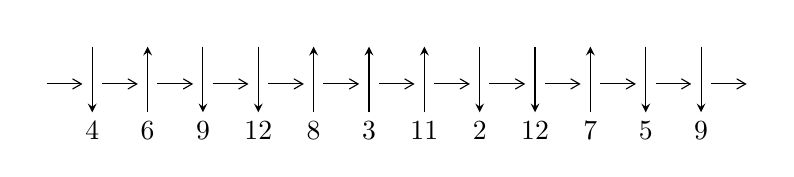
\begin{tikzpicture}[x=20pt, y=17pt]
	% nodes
	\node (C0) at (0, 0) {};
	\node (C1) at (1, 0) {};
	\node (C1U) at (1, +1) {};
	\node (C1D) at (1, -1) {4};

	\node (C2) at (2, 0) {};
	\node (C2U) at (2, +1) {};
	\node (C2D) at (2, -1) {6};

	\node (C3) at (3, 0) {};
	\node (C3U) at (3, +1) {};
	\node (C3D) at (3, -1) {9};

	\node (C4) at (4, 0) {};
	\node (C4U) at (4, +1) {};
	\node (C4D) at (4, -1) {12};

	\node (C5) at (5, 0) {};
	\node (C5U) at (5, +1) {};
	\node (C5D) at (5, -1) {8};

	\node (C6) at (6, 0) {};
	\node (C6U) at (6, +1) {};
	\node (C6D) at (6, -1) {3};

	\node (C7) at (7, 0) {};
	\node (C7U) at (7, +1) {};
	\node (C7D) at (7, -1) {11};

	\node (C8) at (8, 0) {};
	\node (C8U) at (8, +1) {};
	\node (C8D) at (8, -1) {2};

	\node (C9) at (9, 0) {};
	\node (C9U) at (9, +1) {};
	\node (C9D) at (9, -1) {12};

	\node (C10) at (10, 0) {};
	\node (C10U) at (10, +1) {};
	\node (C10D) at (10, -1) {7};

	\node (C11) at (11, 0) {};
	\node (C11U) at (11, +1) {};
	\node (C11D) at (11, -1) {5};

	\node (C12) at (12, 0) {};
	\node (C12U) at (12, +1) {};
	\node (C12D) at (12, -1) {9};
	\node (C13) at (13, 0) {};

	% arrows
	\draw[->,>={angle 60}]
	(C0) edge (C1) (C1) edge (C2) (C2) edge (C3) (C3) edge (C4) (C4) edge (C5) (C5) edge (C6) (C6) edge (C7) (C7) edge (C8) (C8) edge (C9) (C9) edge (C10) (C10) edge (C11) (C11) edge (C12) (C12) edge (C13) ;	\draw[->,>=stealth]
	(C1U) edge (C1D) (C2D) edge (C2U) (C3U) edge (C3D) (C4U) edge (C4D) (C5D) edge (C5U) (C6D) edge (C6U) (C7D) edge (C7U) (C8U) edge (C8D) (C9U) edge (C9D) (C10D) edge (C10U) (C11U) edge (C11D) (C12U) edge (C12D) ;
	\end{tikzpicture} \\
\hhline{~~} \\& 
\textbf{Solving Sequence} \\ \cline{2-2} 
 &
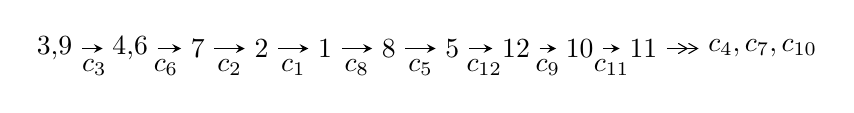
\begin{tikzpicture}[x=23pt, y=7pt]
	% node
	\node (A0) at (-1/8, 0) {3,9};
	\node (A1) at (17/16, 0) {4,6};
	\node (A2) at (17/8, 0) {7};
	\node (A3) at (25/8, 0) {2};
	\node (A4) at (33/8, 0) {1};
	\node (A5) at (41/8, 0) {8};
	\node (A6) at (49/8, 0) {5};
	\node (A7) at (57/8, 0) {12};
	\node (A8) at (65/8, 0) {10};
	\node (A9) at (73/8, 0) {11};
	\node (C1) at (1/2, -1) {$c_{3}$};
	\node (C2) at (13/8, -1) {$c_{6}$};
	\node (C3) at (21/8, -1) {$c_{2}$};
	\node (C4) at (29/8, -1) {$c_{1}$};
	\node (C5) at (37/8, -1) {$c_{8}$};
	\node (C6) at (45/8, -1) {$c_{5}$};
	\node (C7) at (53/8, -1) {$c_{12}$};
	\node (C8) at (61/8, -1) {$c_{9}$};
	\node (C9) at (69/8, -1) {$c_{11}$};
	\node (A10) at (11, 0) {$c_{4},c_{7},c_{10}$};

	% edge
	\draw[->,>=stealth]	
	(A0) edge (A1) (A1) edge (A2) (A2) edge (A3) (A3) edge (A4) (A4) edge (A5) (A5) edge (A6) (A6) edge (A7) (A7) edge (A8) (A8) edge (A9) ;
	\draw[->>,>={angle 60}]	
	(A9) edge (A10);
\end{tikzpicture} \\ 

\end{tabular} \\

\footnotetext{
The image of knot diagram is generated by the software ``\textbf{Draw programme}" developed by Andrew Bartholomew(\url{http://www.layer8.co.uk/maths/draw/index.htm\#Running-draw}), where we modified some parts for our purpose(\url{https://github.com/CATsTAILs/LinksPainter}).
}\phantom \\ \newline 
\centering \textbf{Ideals for irreducible components\footnotemark of $X_{\text{par}}$} 
 
\begin{align*}
I^u_{1}&=\langle 
155164409 u^{19}-1173171752 u^{18}+\cdots+19656063 b+4652516609,\\
\phantom{I^u_{1}}&\phantom{= \langle  }3194027005 u^{19}-23918980957 u^{18}+\cdots+864866772 a+84007929151,\\
\phantom{I^u_{1}}&\phantom{= \langle  }u^{20}-9 u^{19}+\cdots-101 u-44\rangle \\
I^u_{2}&=\langle 
1153398772571 u^{26} a-27659986158013 u^{26}+\cdots+47932282550416 a+517986614105786,\\
\phantom{I^u_{2}}&\phantom{= \langle  }6.62034\times10^{14} a u^{26}+1.26437\times10^{15} u^{26}+\cdots-4.24307\times10^{15} a-1.06993\times10^{16},\;u^{27}+4 u^{26}+\cdots-16 u+1\rangle \\
I^u_{3}&=\langle 
b+u-2,\;2 u^3-12 u^2+5 a+19 u-7,\;u^4-6 u^3+12 u^2-11 u+5\rangle \\
I^u_{4}&=\langle 
u^{10} a+2 u^{11}+\cdots- a-3,\;2 u^{11} a+4 u^{11}+\cdots-3 a+10,\\
\phantom{I^u_{4}}&\phantom{= \langle  }u^{12}+3 u^{11}-2 u^{10}-14 u^9-7 u^8+19 u^7+20 u^6-4 u^5-13 u^4-7 u^3+4 u+1\rangle \\
\\
\end{align*}
\raggedright * 4 irreducible components of $\dim_{\mathbb{C}}=0$, with total 102 representations.\\
\footnotetext{All coefficients of polynomials are rational numbers. But the coefficients are sometimes approximated in decimal forms when there is not enough margin.}
\newpage
\renewcommand{\arraystretch}{1}
\centering \section*{I. $I^u_{1}= \langle 1.55\times10^{8} u^{19}-1.17\times10^{9} u^{18}+\cdots+1.97\times10^{7} b+4.65\times10^{9},\;3.19\times10^{9} u^{19}-2.39\times10^{10} u^{18}+\cdots+8.65\times10^{8} a+8.40\times10^{10},\;u^{20}-9 u^{19}+\cdots-101 u-44 \rangle$}
\flushleft \textbf{(i) Arc colorings}\\
\begin{tabular}{m{7pt} m{180pt} m{7pt} m{180pt} }
\flushright $a_{3}=$&$\begin{pmatrix}1\\0\end{pmatrix}$ \\
\flushright $a_{9}=$&$\begin{pmatrix}0\\u\end{pmatrix}$ \\
\flushright $a_{4}=$&$\begin{pmatrix}1\\u^2\end{pmatrix}$ \\
\flushright $a_{6}=$&$\begin{pmatrix}-3.69309 u^{19}+27.6563 u^{18}+\cdots-289.384 u-97.1340\\-7.89397 u^{19}+59.6850 u^{18}+\cdots-701.033 u-236.696\end{pmatrix}$ \\
\flushright $a_{7}=$&$\begin{pmatrix}-11.5871 u^{19}+87.3412 u^{18}+\cdots-990.417 u-333.830\\-7.89397 u^{19}+59.6850 u^{18}+\cdots-701.033 u-236.696\end{pmatrix}$ \\
\flushright $a_{2}=$&$\begin{pmatrix}-0.729812 u^{19}+5.09498 u^{18}+\cdots-10.5444 u-0.980246\\-3.00124 u^{19}+23.1501 u^{18}+\cdots-293.563 u-98.7110\end{pmatrix}$ \\
\flushright $a_{1}=$&$\begin{pmatrix}-0.770109 u^{19}+6.89068 u^{18}+\cdots-123.191 u-34.8650\\1.39273 u^{19}-6.70756 u^{18}+\cdots-150.601 u-35.6579\end{pmatrix}$ \\
\flushright $a_{8}=$&$\begin{pmatrix}1.32525 u^{19}-10.3344 u^{18}+\cdots+119.923 u+43.4460\\-2.61701 u^{19}+19.7532 u^{18}+\cdots-222.509 u-77.4331\end{pmatrix}$ \\
\flushright $a_{5}=$&$\begin{pmatrix}-3.35278 u^{19}+25.4969 u^{18}+\cdots-322.784 u-103.076\\-4.67803 u^{19}+35.8313 u^{18}+\cdots-442.706 u-147.522\end{pmatrix}$ \\
\flushright $a_{12}=$&$\begin{pmatrix}-0.770109 u^{19}+6.89068 u^{18}+\cdots-123.191 u-34.8650\\-0.0402972 u^{19}+1.79570 u^{18}+\cdots-112.646 u-33.8848\end{pmatrix}$ \\
\flushright $a_{10}=$&$\begin{pmatrix}-7.78475 u^{19}+58.9253 u^{18}+\cdots-701.929 u-238.453\\-11.1375 u^{19}+84.4222 u^{18}+\cdots-1023.71 u-342.529\end{pmatrix}$ \\
\flushright $a_{11}=$&$\begin{pmatrix}-4.05370 u^{19}+30.6802 u^{18}+\cdots-397.822 u-137.762\\-8.13629 u^{19}+61.2722 u^{18}+\cdots-730.150 u-243.818\end{pmatrix}$\\&\end{tabular}
\flushleft \textbf{(ii) Obstruction class $= -1$}\\~\\
\flushleft \textbf{(iii) Cusp Shapes $= \frac{1862218903}{19656063} u^{19}-\frac{13770753601}{19656063} u^{18}+\cdots+\frac{47665991273}{6552021} u+\frac{49632160054}{19656063}$}\\~\\
\newpage\renewcommand{\arraystretch}{1}
\flushleft \textbf{(iv) u-Polynomials at the component}\newline \\
\begin{tabular}{m{50pt}|m{274pt}}
Crossings & \hspace{64pt}u-Polynomials at each crossing \\
\hline $$\begin{aligned}c_{1},c_{9},c_{12}\end{aligned}$$&$\begin{aligned}
&u^{20}+3 u^{19}+\cdots+7 u+1
\end{aligned}$\\
\hline $$\begin{aligned}c_{2},c_{6},c_{7}\\c_{10}\end{aligned}$$&$\begin{aligned}
&u^{20}-3 u^{18}+\cdots-2 u-1
\end{aligned}$\\
\hline $$\begin{aligned}c_{3}\end{aligned}$$&$\begin{aligned}
&u^{20}-9 u^{19}+\cdots-101 u-44
\end{aligned}$\\
\hline $$\begin{aligned}c_{4},c_{8},c_{11}\end{aligned}$$&$\begin{aligned}
&u^{20}- u^{19}+\cdots+u-1
\end{aligned}$\\
\hline $$\begin{aligned}c_{5}\end{aligned}$$&$\begin{aligned}
&u^{20}+4 u^{19}+\cdots+371 u+44
\end{aligned}$\\
\hline
\end{tabular}\\~\\
\newpage\renewcommand{\arraystretch}{1}
\flushleft \textbf{(v) Riley Polynomials at the component}\newline \\
\begin{tabular}{m{50pt}|m{274pt}}
Crossings & \hspace{64pt}Riley Polynomials at each crossing \\
\hline $$\begin{aligned}c_{1},c_{9},c_{12}\end{aligned}$$&$\begin{aligned}
&y^{20}-31 y^{19}+\cdots-53 y+1
\end{aligned}$\\
\hline $$\begin{aligned}c_{2},c_{6},c_{7}\\c_{10}\end{aligned}$$&$\begin{aligned}
&y^{20}-6 y^{19}+\cdots-2 y+1
\end{aligned}$\\
\hline $$\begin{aligned}c_{3}\end{aligned}$$&$\begin{aligned}
&y^{20}-29 y^{19}+\cdots-23841 y+1936
\end{aligned}$\\
\hline $$\begin{aligned}c_{4},c_{8},c_{11}\end{aligned}$$&$\begin{aligned}
&y^{20}+9 y^{19}+\cdots+3 y+1
\end{aligned}$\\
\hline $$\begin{aligned}c_{5}\end{aligned}$$&$\begin{aligned}
&y^{20}-22 y^{19}+\cdots-10041 y+1936
\end{aligned}$\\
\hline
\end{tabular}\\~\\
\newpage\flushleft \textbf{(vi) Complex Volumes and Cusp Shapes}
$$\begin{array}{c|c|c}  
\text{Solutions to }I^u_{1}& \I (\text{vol} + \sqrt{-1}CS) & \text{Cusp shape}\\
 \hline 
\begin{aligned}
u &= -1.052670 + 0.214579 I \\
a &= \phantom{-}0.32175 - 1.92778 I \\
b &= -0.836827 - 0.543539 I\end{aligned}
 & \phantom{-}6.83483 + 4.33332 I & \phantom{-}0.05876 - 7.63423 I \\ \hline\begin{aligned}
u &= -1.052670 - 0.214579 I \\
a &= \phantom{-}0.32175 + 1.92778 I \\
b &= -0.836827 + 0.543539 I\end{aligned}
 & \phantom{-}6.83483 - 4.33332 I & \phantom{-}0.05876 + 7.63423 I \\ \hline\begin{aligned}
u &= \phantom{-}1.120110 + 0.346275 I \\
a &= -0.233306 - 0.424229 I \\
b &= -0.38707 - 1.48766 I\end{aligned}
 & -5.30551 - 1.26066 I & \phantom{-}2.12940 + 5.78685 I \\ \hline\begin{aligned}
u &= \phantom{-}1.120110 - 0.346275 I \\
a &= -0.233306 + 0.424229 I \\
b &= -0.38707 + 1.48766 I\end{aligned}
 & -5.30551 + 1.26066 I & \phantom{-}2.12940 - 5.78685 I \\ \hline\begin{aligned}
u &= -0.476182 + 0.251897 I \\
a &= \phantom{-}0.298266 + 0.199444 I \\
b &= \phantom{-}0.127716 - 0.483656 I\end{aligned}
 & -0.934143 + 0.731157 I & -6.62873 - 3.56102 I \\ \hline\begin{aligned}
u &= -0.476182 - 0.251897 I \\
a &= \phantom{-}0.298266 - 0.199444 I \\
b &= \phantom{-}0.127716 + 0.483656 I\end{aligned}
 & -0.934143 - 0.731157 I & -6.62873 + 3.56102 I \\ \hline\begin{aligned}
u &= \phantom{-}1.46200 + 0.11516 I \\
a &= -0.105955 + 0.364783 I \\
b &= \phantom{-}0.313911 + 0.848453 I\end{aligned}
 & -7.00266 + 1.06770 I & -8.57959 - 5.53529 I \\ \hline\begin{aligned}
u &= \phantom{-}1.46200 - 0.11516 I \\
a &= -0.105955 - 0.364783 I \\
b &= \phantom{-}0.313911 - 0.848453 I\end{aligned}
 & -7.00266 - 1.06770 I & -8.57959 + 5.53529 I \\ \hline\begin{aligned}
u &= -0.42309 + 1.47138 I \\
a &= -1.165830 + 0.209425 I \\
b &= \phantom{-}1.44769 + 0.49745 I\end{aligned}
 & \phantom{-}7.84975 + 9.25606 I & \phantom{-}2.98645 - 8.19728 I \\ \hline\begin{aligned}
u &= -0.42309 - 1.47138 I \\
a &= -1.165830 - 0.209425 I \\
b &= \phantom{-}1.44769 - 0.49745 I\end{aligned}
 & \phantom{-}7.84975 - 9.25606 I & \phantom{-}2.98645 + 8.19728 I\\
 \hline 
 \end{array}$$\newpage$$\begin{array}{c|c|c}  
\text{Solutions to }I^u_{1}& \I (\text{vol} + \sqrt{-1}CS) & \text{Cusp shape}\\
 \hline 
\begin{aligned}
u &= \phantom{-}1.44287 + 0.52695 I \\
a &= \phantom{-}1.215020 + 0.143277 I \\
b &= -0.794041 - 0.102232 I\end{aligned}
 & \phantom{-}2.39136 + 0.46763 I & \phantom{-}16.5681 - 6.4930 I \\ \hline\begin{aligned}
u &= \phantom{-}1.44287 - 0.52695 I \\
a &= \phantom{-}1.215020 - 0.143277 I \\
b &= -0.794041 + 0.102232 I\end{aligned}
 & \phantom{-}2.39136 - 0.46763 I & \phantom{-}16.5681 + 6.4930 I \\ \hline\begin{aligned}
u &= -0.374420 + 0.266879 I \\
a &= -3.88796 + 1.78468 I \\
b &= \phantom{-}0.790015 - 0.335634 I\end{aligned}
 & \phantom{-}9.03012 - 2.73757 I & \phantom{-}11.18044 + 1.41623 I \\ \hline\begin{aligned}
u &= -0.374420 - 0.266879 I \\
a &= -3.88796 - 1.78468 I \\
b &= \phantom{-}0.790015 + 0.335634 I\end{aligned}
 & \phantom{-}9.03012 + 2.73757 I & \phantom{-}11.18044 - 1.41623 I \\ \hline\begin{aligned}
u &= \phantom{-}1.67183\phantom{ +0.000000I} \\
a &= \phantom{-}0.0164989\phantom{ +0.000000I} \\
b &= \phantom{-}0.556210\phantom{ +0.000000I}\end{aligned}
 & -7.42843\phantom{ +0.000000I} & \phantom{-}21.0830\phantom{ +0.000000I} \\ \hline\begin{aligned}
u &= \phantom{-}1.64455 + 0.32821 I \\
a &= -0.97484 - 1.07134 I \\
b &= \phantom{-}0.955066 - 0.584622 I\end{aligned}
 & -3.92374 - 8.34608 I & \phantom{-0.000000 -}0. + 8.57009 I \\ \hline\begin{aligned}
u &= \phantom{-}1.64455 - 0.32821 I \\
a &= -0.97484 + 1.07134 I \\
b &= \phantom{-}0.955066 + 0.584622 I\end{aligned}
 & -3.92374 + 8.34608 I & \phantom{-0.000000 } 0. - 8.57009 I \\ \hline\begin{aligned}
u &= \phantom{-}1.66385 + 0.49105 I \\
a &= \phantom{-}0.747318 + 0.938443 I \\
b &= -1.33112 + 0.78381 I\end{aligned}
 & \phantom{-}1.0956 - 16.1913 I & \phantom{-}1.21980 + 7.93611 I \\ \hline\begin{aligned}
u &= \phantom{-}1.66385 - 0.49105 I \\
a &= \phantom{-}0.747318 - 0.938443 I \\
b &= -1.33112 - 0.78381 I\end{aligned}
 & \phantom{-}1.0956 + 16.1913 I & \phantom{-}1.21980 - 7.93611 I \\ \hline\begin{aligned}
u &= -2.68586\phantom{ +0.000000I} \\
a &= \phantom{-}0.713636\phantom{ +0.000000I} \\
b &= -1.12689\phantom{ +0.000000I}\end{aligned}
 & \phantom{-}3.80648\phantom{ +0.000000I} & \phantom{-0.000000 } 0\\
 \hline 
 \end{array}$$\newpage\newpage\renewcommand{\arraystretch}{1}
\centering \section*{II. $I^u_{2}= \langle 1.15\times10^{12} a u^{26}-2.77\times10^{13} u^{26}+\cdots+4.79\times10^{13} a+5.18\times10^{14},\;6.62\times10^{14} a u^{26}+1.26\times10^{15} u^{26}+\cdots-4.24\times10^{15} a-1.07\times10^{16},\;u^{27}+4 u^{26}+\cdots-16 u+1 \rangle$}
\flushleft \textbf{(i) Arc colorings}\\
\begin{tabular}{m{7pt} m{180pt} m{7pt} m{180pt} }
\flushright $a_{3}=$&$\begin{pmatrix}1\\0\end{pmatrix}$ \\
\flushright $a_{9}=$&$\begin{pmatrix}0\\u\end{pmatrix}$ \\
\flushright $a_{4}=$&$\begin{pmatrix}1\\u^2\end{pmatrix}$ \\
\flushright $a_{6}=$&$\begin{pmatrix}a\\-0.0242410 a u^{26}+0.581330 u^{26}+\cdots-1.00739 a-10.8865\end{pmatrix}$ \\
\flushright $a_{7}=$&$\begin{pmatrix}-0.0242410 a u^{26}+0.581330 u^{26}+\cdots-0.00739376 a-10.8865\\-0.0242410 a u^{26}+0.581330 u^{26}+\cdots-1.00739 a-10.8865\end{pmatrix}$ \\
\flushright $a_{2}=$&$\begin{pmatrix}-1.08669 a u^{26}+0.00739376 u^{26}+\cdots+7.02849 a+7.42850\\-0.0360384 a u^{26}-1.26454 u^{26}+\cdots-0.689023 a+8.59574\end{pmatrix}$ \\
\flushright $a_{1}=$&$\begin{pmatrix}-0.841478 a u^{26}-u^{26}+\cdots+6.18701 a+16\\0.337969 a u^{26}-1.00739 u^{26}+\cdots-0.596266 a+8.57150\end{pmatrix}$ \\
\flushright $a_{8}=$&$\begin{pmatrix}-1.50664 a u^{26}-2.66029 u^{26}+\cdots+10.2782 a+26.5660\\-0.242104 a u^{26}-1.76324 u^{26}+\cdots+1.68247 a+6.29618\end{pmatrix}$ \\
\flushright $a_{5}=$&$\begin{pmatrix}0.513982 a u^{26}-4.80755 u^{26}+\cdots-2.50550 a+27.3198\\0.513982 a u^{26}+1.68297 u^{26}+\cdots-2.50550 a-9.53524\end{pmatrix}$ \\
\flushright $a_{12}=$&$\begin{pmatrix}-0.841478 a u^{26}-u^{26}+\cdots+6.18701 a+16\\0.245212 a u^{26}-1.00739 u^{26}+\cdots-0.841478 a+8.57150\end{pmatrix}$ \\
\flushright $a_{10}=$&$\begin{pmatrix}2.50550 a u^{26}+4.15537 u^{26}+\cdots-10.7922 a-38.4438\\0.398816 u^{26}+2.23271 u^{25}+\cdots+57.1829 u-5.41613\end{pmatrix}$ \\
\flushright $a_{11}=$&$\begin{pmatrix}1.92417 a u^{26}+3.36740 u^{26}+\cdots+0.0943422 a-27.9026\\-0.396547 u^{26}+0.153675 u^{25}+\cdots+32.0090 u-1.30351\end{pmatrix}$\\&\end{tabular}
\flushleft \textbf{(ii) Obstruction class $= -1$}\\~\\
\flushleft \textbf{(iii) Cusp Shapes $= \frac{195093488669178}{47580483876995} u^{26}+\frac{621166284588117}{47580483876995} u^{25}+\cdots+\frac{10739526635696416}{47580483876995} u-\frac{1670488305527964}{47580483876995}$}\\~\\
\newpage\renewcommand{\arraystretch}{1}
\flushleft \textbf{(iv) u-Polynomials at the component}\newline \\
\begin{tabular}{m{50pt}|m{274pt}}
Crossings & \hspace{64pt}u-Polynomials at each crossing \\
\hline $$\begin{aligned}c_{1},c_{9},c_{12}\end{aligned}$$&$\begin{aligned}
&u^{54}-9 u^{53}+\cdots-817482 u+44911
\end{aligned}$\\
\hline $$\begin{aligned}c_{2},c_{6},c_{7}\\c_{10}\end{aligned}$$&$\begin{aligned}
&u^{54}-2 u^{53}+\cdots-7504 u+1667
\end{aligned}$\\
\hline $$\begin{aligned}c_{3}\end{aligned}$$&$\begin{aligned}
&(u^{27}+4 u^{26}+\cdots-16 u+1)^{2}
\end{aligned}$\\
\hline $$\begin{aligned}c_{4},c_{8},c_{11}\end{aligned}$$&$\begin{aligned}
&u^{54}+3 u^{53}+\cdots-7068 u+1763
\end{aligned}$\\
\hline $$\begin{aligned}c_{5}\end{aligned}$$&$\begin{aligned}
&(u^{27}-2 u^{26}+\cdots-67 u+47)^{2}
\end{aligned}$\\
\hline
\end{tabular}\\~\\
\newpage\renewcommand{\arraystretch}{1}
\flushleft \textbf{(v) Riley Polynomials at the component}\newline \\
\begin{tabular}{m{50pt}|m{274pt}}
Crossings & \hspace{64pt}Riley Polynomials at each crossing \\
\hline $$\begin{aligned}c_{1},c_{9},c_{12}\end{aligned}$$&$\begin{aligned}
&y^{54}-53 y^{53}+\cdots+26272962362 y+2016997921
\end{aligned}$\\
\hline $$\begin{aligned}c_{2},c_{6},c_{7}\\c_{10}\end{aligned}$$&$\begin{aligned}
&y^{54}-28 y^{53}+\cdots-34895734 y+2778889
\end{aligned}$\\
\hline $$\begin{aligned}c_{3}\end{aligned}$$&$\begin{aligned}
&(y^{27}-30 y^{26}+\cdots+108 y-1)^{2}
\end{aligned}$\\
\hline $$\begin{aligned}c_{4},c_{8},c_{11}\end{aligned}$$&$\begin{aligned}
&y^{54}+27 y^{53}+\cdots+38637652 y+3108169
\end{aligned}$\\
\hline $$\begin{aligned}c_{5}\end{aligned}$$&$\begin{aligned}
&(y^{27}-20 y^{26}+\cdots+14171 y-2209)^{2}
\end{aligned}$\\
\hline
\end{tabular}\\~\\
\newpage\flushleft \textbf{(vi) Complex Volumes and Cusp Shapes}
$$\begin{array}{c|c|c}  
\text{Solutions to }I^u_{2}& \I (\text{vol} + \sqrt{-1}CS) & \text{Cusp shape}\\
 \hline 
\begin{aligned}
u &= -0.158532 + 0.935582 I \\
a &= -1.50310 + 0.50723 I \\
b &= \phantom{-}1.316050 - 0.206467 I\end{aligned}
 & \phantom{-}2.66520 - 3.11494 I & \phantom{-}4.06258 + 4.43870 I \\ \hline\begin{aligned}
u &= -0.158532 + 0.935582 I \\
a &= -0.232784 + 0.158230 I \\
b &= -0.125783 + 1.310910 I\end{aligned}
 & \phantom{-}2.66520 - 3.11494 I & \phantom{-}4.06258 + 4.43870 I \\ \hline\begin{aligned}
u &= -0.158532 - 0.935582 I \\
a &= -1.50310 - 0.50723 I \\
b &= \phantom{-}1.316050 + 0.206467 I\end{aligned}
 & \phantom{-}2.66520 + 3.11494 I & \phantom{-}4.06258 - 4.43870 I \\ \hline\begin{aligned}
u &= -0.158532 - 0.935582 I \\
a &= -0.232784 - 0.158230 I \\
b &= -0.125783 - 1.310910 I\end{aligned}
 & \phantom{-}2.66520 + 3.11494 I & \phantom{-}4.06258 - 4.43870 I \\ \hline\begin{aligned}
u &= \phantom{-}1.07088\phantom{ +0.000000I} \\
a &= \phantom{-}0.20349 + 1.69086 I \\
b &= -1.039390 + 0.501438 I\end{aligned}
 & \phantom{-}7.61014\phantom{ +0.000000I} & \phantom{-}2.10720\phantom{ +0.000000I} \\ \hline\begin{aligned}
u &= \phantom{-}1.07088\phantom{ +0.000000I} \\
a &= \phantom{-}0.20349 - 1.69086 I \\
b &= -1.039390 - 0.501438 I\end{aligned}
 & \phantom{-}7.61014\phantom{ +0.000000I} & \phantom{-}2.10720\phantom{ +0.000000I} \\ \hline\begin{aligned}
u &= \phantom{-}0.221976 + 0.825159 I \\
a &= \phantom{-}0.865041 - 0.769539 I \\
b &= -0.188178 - 0.427579 I\end{aligned}
 & \phantom{-}1.85443 + 1.12451 I & \phantom{-}2.23685 + 3.40792 I \\ \hline\begin{aligned}
u &= \phantom{-}0.221976 + 0.825159 I \\
a &= \phantom{-}1.56832 + 0.15522 I \\
b &= -1.056960 - 0.253260 I\end{aligned}
 & \phantom{-}1.85443 + 1.12451 I & \phantom{-}2.23685 + 3.40792 I \\ \hline\begin{aligned}
u &= \phantom{-}0.221976 - 0.825159 I \\
a &= \phantom{-}0.865041 + 0.769539 I \\
b &= -0.188178 + 0.427579 I\end{aligned}
 & \phantom{-}1.85443 - 1.12451 I & \phantom{-}2.23685 - 3.40792 I \\ \hline\begin{aligned}
u &= \phantom{-}0.221976 - 0.825159 I \\
a &= \phantom{-}1.56832 - 0.15522 I \\
b &= -1.056960 + 0.253260 I\end{aligned}
 & \phantom{-}1.85443 - 1.12451 I & \phantom{-}2.23685 - 3.40792 I\\
 \hline 
 \end{array}$$\newpage$$\begin{array}{c|c|c}  
\text{Solutions to }I^u_{2}& \I (\text{vol} + \sqrt{-1}CS) & \text{Cusp shape}\\
 \hline 
\begin{aligned}
u &= -0.772781 + 0.145831 I \\
a &= -0.955249 + 0.172273 I \\
b &= \phantom{-}0.942406 - 0.743444 I\end{aligned}
 & \phantom{-}5.86045 + 0.50074 I & -0.026133 - 1.385067 I \\ \hline\begin{aligned}
u &= -0.772781 + 0.145831 I \\
a &= -0.03004 - 1.56141 I \\
b &= -0.956615 - 0.919647 I\end{aligned}
 & \phantom{-}5.86045 + 0.50074 I & -0.026133 - 1.385067 I \\ \hline\begin{aligned}
u &= -0.772781 - 0.145831 I \\
a &= -0.955249 - 0.172273 I \\
b &= \phantom{-}0.942406 + 0.743444 I\end{aligned}
 & \phantom{-}5.86045 - 0.50074 I & -0.026133 + 1.385067 I \\ \hline\begin{aligned}
u &= -0.772781 - 0.145831 I \\
a &= -0.03004 + 1.56141 I \\
b &= -0.956615 + 0.919647 I\end{aligned}
 & \phantom{-}5.86045 - 0.50074 I & -0.026133 + 1.385067 I \\ \hline\begin{aligned}
u &= \phantom{-}0.732746 + 0.037797 I \\
a &= -0.197320 + 0.642818 I \\
b &= \phantom{-}1.097490 - 0.609563 I\end{aligned}
 & \phantom{-}6.70782 - 6.19371 I & \phantom{-}1.04615 + 5.14040 I \\ \hline\begin{aligned}
u &= \phantom{-}0.732746 + 0.037797 I \\
a &= \phantom{-}0.39411 + 1.87802 I \\
b &= -1.136770 + 0.758571 I\end{aligned}
 & \phantom{-}6.70782 - 6.19371 I & \phantom{-}1.04615 + 5.14040 I \\ \hline\begin{aligned}
u &= \phantom{-}0.732746 - 0.037797 I \\
a &= -0.197320 - 0.642818 I \\
b &= \phantom{-}1.097490 + 0.609563 I\end{aligned}
 & \phantom{-}6.70782 + 6.19371 I & \phantom{-}1.04615 - 5.14040 I \\ \hline\begin{aligned}
u &= \phantom{-}0.732746 - 0.037797 I \\
a &= \phantom{-}0.39411 - 1.87802 I \\
b &= -1.136770 - 0.758571 I\end{aligned}
 & \phantom{-}6.70782 + 6.19371 I & \phantom{-}1.04615 - 5.14040 I \\ \hline\begin{aligned}
u &= -1.41462 + 0.08838 I \\
a &= \phantom{-}0.262151 - 0.521305 I \\
b &= \phantom{-}0.744839 - 1.008240 I\end{aligned}
 & -3.85325 - 2.16315 I & \phantom{-}0.43125 + 2.34406 I \\ \hline\begin{aligned}
u &= -1.41462 + 0.08838 I \\
a &= \phantom{-}0.94161 + 1.25020 I \\
b &= -0.893423 + 0.347194 I\end{aligned}
 & -3.85325 - 2.16315 I & \phantom{-}0.43125 + 2.34406 I\\
 \hline 
 \end{array}$$\newpage$$\begin{array}{c|c|c}  
\text{Solutions to }I^u_{2}& \I (\text{vol} + \sqrt{-1}CS) & \text{Cusp shape}\\
 \hline 
\begin{aligned}
u &= -1.41462 - 0.08838 I \\
a &= \phantom{-}0.262151 + 0.521305 I \\
b &= \phantom{-}0.744839 + 1.008240 I\end{aligned}
 & -3.85325 + 2.16315 I & \phantom{-}0.43125 - 2.34406 I \\ \hline\begin{aligned}
u &= -1.41462 - 0.08838 I \\
a &= \phantom{-}0.94161 - 1.25020 I \\
b &= -0.893423 - 0.347194 I\end{aligned}
 & -3.85325 + 2.16315 I & \phantom{-}0.43125 - 2.34406 I \\ \hline\begin{aligned}
u &= \phantom{-}0.96419 + 1.06250 I \\
a &= -0.777537 - 0.509617 I \\
b &= \phantom{-}1.49984 - 0.06654 I\end{aligned}
 & \phantom{-}7.39896 - 3.81582 I & \phantom{-}3.19122 + 3.12687 I \\ \hline\begin{aligned}
u &= \phantom{-}0.96419 + 1.06250 I \\
a &= \phantom{-}0.996480 + 0.564354 I \\
b &= -1.52086 + 0.54966 I\end{aligned}
 & \phantom{-}7.39896 - 3.81582 I & \phantom{-}3.19122 + 3.12687 I \\ \hline\begin{aligned}
u &= \phantom{-}0.96419 - 1.06250 I \\
a &= -0.777537 + 0.509617 I \\
b &= \phantom{-}1.49984 + 0.06654 I\end{aligned}
 & \phantom{-}7.39896 + 3.81582 I & \phantom{-}3.19122 - 3.12687 I \\ \hline\begin{aligned}
u &= \phantom{-}0.96419 - 1.06250 I \\
a &= \phantom{-}0.996480 - 0.564354 I \\
b &= -1.52086 - 0.54966 I\end{aligned}
 & \phantom{-}7.39896 + 3.81582 I & \phantom{-}3.19122 - 3.12687 I \\ \hline\begin{aligned}
u &= \phantom{-}1.46227 + 0.17089 I \\
a &= -0.70585 - 1.22803 I \\
b &= \phantom{-}1.080150 - 0.757376 I\end{aligned}
 & -2.64494 - 4.30028 I & \phantom{-}1.62045 + 0.54924 I \\ \hline\begin{aligned}
u &= \phantom{-}1.46227 + 0.17089 I \\
a &= \phantom{-}1.11356 - 1.22226 I \\
b &= -0.794850 - 0.366906 I\end{aligned}
 & -2.64494 - 4.30028 I & \phantom{-}1.62045 + 0.54924 I \\ \hline\begin{aligned}
u &= \phantom{-}1.46227 - 0.17089 I \\
a &= -0.70585 + 1.22803 I \\
b &= \phantom{-}1.080150 + 0.757376 I\end{aligned}
 & -2.64494 + 4.30028 I & \phantom{-}1.62045 - 0.54924 I \\ \hline\begin{aligned}
u &= \phantom{-}1.46227 - 0.17089 I \\
a &= \phantom{-}1.11356 + 1.22226 I \\
b &= -0.794850 + 0.366906 I\end{aligned}
 & -2.64494 + 4.30028 I & \phantom{-}1.62045 - 0.54924 I\\
 \hline 
 \end{array}$$\newpage$$\begin{array}{c|c|c}  
\text{Solutions to }I^u_{2}& \I (\text{vol} + \sqrt{-1}CS) & \text{Cusp shape}\\
 \hline 
\begin{aligned}
u &= -1.53479\phantom{ +0.000000I} \\
a &= \phantom{-}0.414758 + 0.269711 I \\
b &= -1.024280 - 0.077414 I\end{aligned}
 & \phantom{-}3.41879\phantom{ +0.000000I} & \phantom{-}6.41080\phantom{ +0.000000I} \\ \hline\begin{aligned}
u &= -1.53479\phantom{ +0.000000I} \\
a &= \phantom{-}0.414758 - 0.269711 I \\
b &= -1.024280 + 0.077414 I\end{aligned}
 & \phantom{-}3.41879\phantom{ +0.000000I} & \phantom{-}6.41080\phantom{ +0.000000I} \\ \hline\begin{aligned}
u &= -1.46424 + 0.50584 I \\
a &= \phantom{-}0.865744 - 0.882179 I \\
b &= -1.37593 - 0.68985 I\end{aligned}
 & -1.70679 + 8.63753 I & \phantom{-}0.70129 - 5.57252 I \\ \hline\begin{aligned}
u &= -1.46424 + 0.50584 I \\
a &= -0.222321 + 0.420033 I \\
b &= -0.51373 + 1.37153 I\end{aligned}
 & -1.70679 + 8.63753 I & \phantom{-}0.70129 - 5.57252 I \\ \hline\begin{aligned}
u &= -1.46424 - 0.50584 I \\
a &= \phantom{-}0.865744 + 0.882179 I \\
b &= -1.37593 + 0.68985 I\end{aligned}
 & -1.70679 - 8.63753 I & \phantom{-}0.70129 + 5.57252 I \\ \hline\begin{aligned}
u &= -1.46424 - 0.50584 I \\
a &= -0.222321 - 0.420033 I \\
b &= -0.51373 - 1.37153 I\end{aligned}
 & -1.70679 - 8.63753 I & \phantom{-}0.70129 + 5.57252 I \\ \hline\begin{aligned}
u &= \phantom{-}1.60572 + 0.14635 I \\
a &= \phantom{-}0.143649 + 0.671229 I \\
b &= \phantom{-}0.676206 + 1.121340 I\end{aligned}
 & -3.96610 - 0.49039 I & \phantom{-}2.17660 + 0.87451 I \\ \hline\begin{aligned}
u &= \phantom{-}1.60572 + 0.14635 I \\
a &= -0.032560 + 0.591612 I \\
b &= -0.898818 + 0.272522 I\end{aligned}
 & -3.96610 - 0.49039 I & \phantom{-}2.17660 + 0.87451 I \\ \hline\begin{aligned}
u &= \phantom{-}1.60572 - 0.14635 I \\
a &= \phantom{-}0.143649 - 0.671229 I \\
b &= \phantom{-}0.676206 - 1.121340 I\end{aligned}
 & -3.96610 + 0.49039 I & \phantom{-}2.17660 - 0.87451 I \\ \hline\begin{aligned}
u &= \phantom{-}1.60572 - 0.14635 I \\
a &= -0.032560 - 0.591612 I \\
b &= -0.898818 - 0.272522 I\end{aligned}
 & -3.96610 + 0.49039 I & \phantom{-}2.17660 - 0.87451 I\\
 \hline 
 \end{array}$$\newpage$$\begin{array}{c|c|c}  
\text{Solutions to }I^u_{2}& \I (\text{vol} + \sqrt{-1}CS) & \text{Cusp shape}\\
 \hline 
\begin{aligned}
u &= -1.61132 + 0.29006 I \\
a &= -0.953605 + 0.809181 I \\
b &= \phantom{-}1.074430 + 0.451641 I\end{aligned}
 & -4.62159 + 3.33366 I & \phantom{-0.000000 } 0. - 1.64502 I \\ \hline\begin{aligned}
u &= -1.61132 + 0.29006 I \\
a &= \phantom{-}0.079718 - 0.306892 I \\
b &= \phantom{-}0.745769 - 0.725411 I\end{aligned}
 & -4.62159 + 3.33366 I & \phantom{-0.000000 } 0. - 1.64502 I \\ \hline\begin{aligned}
u &= -1.61132 - 0.29006 I \\
a &= -0.953605 - 0.809181 I \\
b &= \phantom{-}1.074430 - 0.451641 I\end{aligned}
 & -4.62159 - 3.33366 I & \phantom{-0.000000 -}0. + 1.64502 I \\ \hline\begin{aligned}
u &= -1.61132 - 0.29006 I \\
a &= \phantom{-}0.079718 + 0.306892 I \\
b &= \phantom{-}0.745769 + 0.725411 I\end{aligned}
 & -4.62159 - 3.33366 I & \phantom{-0.000000 -}0. + 1.64502 I \\ \hline\begin{aligned}
u &= -1.64260 + 0.12656 I \\
a &= -0.539122 + 1.081180 I \\
b &= \phantom{-}1.193170 + 0.752557 I\end{aligned}
 & -2.09892 + 7.32302 I & \phantom{-}1.91859 - 5.85391 I \\ \hline\begin{aligned}
u &= -1.64260 + 0.12656 I \\
a &= -0.147988 - 0.383193 I \\
b &= -0.958048 - 0.349092 I\end{aligned}
 & -2.09892 + 7.32302 I & \phantom{-}1.91859 - 5.85391 I \\ \hline\begin{aligned}
u &= -1.64260 - 0.12656 I \\
a &= -0.539122 - 1.081180 I \\
b &= \phantom{-}1.193170 - 0.752557 I\end{aligned}
 & -2.09892 - 7.32302 I & \phantom{-}1.91859 + 5.85391 I \\ \hline\begin{aligned}
u &= -1.64260 - 0.12656 I \\
a &= -0.147988 + 0.383193 I \\
b &= -0.958048 + 0.349092 I\end{aligned}
 & -2.09892 - 7.32302 I & \phantom{-}1.91859 + 5.85391 I \\ \hline\begin{aligned}
u &= \phantom{-}0.341878\phantom{ +0.000000I} \\
a &= -0.80620 + 4.25915 I \\
b &= \phantom{-}1.024170 - 0.310510 I\end{aligned}
 & \phantom{-}10.0079\phantom{ +0.000000I} & \phantom{-}6.39560\phantom{ +0.000000I} \\ \hline\begin{aligned}
u &= \phantom{-}0.341878\phantom{ +0.000000I} \\
a &= -0.80620 - 4.25915 I \\
b &= \phantom{-}1.024170 + 0.310510 I\end{aligned}
 & \phantom{-}10.0079\phantom{ +0.000000I} & \phantom{-}6.39560\phantom{ +0.000000I}\\
 \hline 
 \end{array}$$\newpage$$\begin{array}{c|c|c}  
\text{Solutions to }I^u_{2}& \I (\text{vol} + \sqrt{-1}CS) & \text{Cusp shape}\\
 \hline 
\begin{aligned}
u &= \phantom{-}0.1382100 + 0.0296626 I \\
a &= -2.23980 - 1.90608 I \\
b &= -0.676102 + 0.783648 I\end{aligned}
 & \phantom{-}1.15814 - 2.56837 I & -5.68616 + 5.09265 I \\ \hline\begin{aligned}
u &= \phantom{-}0.1382100 + 0.0296626 I \\
a &= -4.00516 - 10.10660 I \\
b &= \phantom{-}0.765217 - 0.171124 I\end{aligned}
 & \phantom{-}1.15814 - 2.56837 I & -5.68616 + 5.09265 I \\ \hline\begin{aligned}
u &= \phantom{-}0.1382100 - 0.0296626 I \\
a &= -2.23980 + 1.90608 I \\
b &= -0.676102 - 0.783648 I\end{aligned}
 & \phantom{-}1.15814 + 2.56837 I & -5.68616 - 5.09265 I \\ \hline\begin{aligned}
u &= \phantom{-}0.1382100 - 0.0296626 I \\
a &= -4.00516 + 10.10660 I \\
b &= \phantom{-}0.765217 + 0.171124 I\end{aligned}
 & \phantom{-}1.15814 + 2.56837 I & -5.68616 - 5.09265 I\\
 \hline 
 \end{array}$$\newpage\newpage\renewcommand{\arraystretch}{1}
\centering \section*{III. $I^u_{3}= \langle b+u-2,\;2 u^3-12 u^2+5 a+19 u-7,\;u^4-6 u^3+12 u^2-11 u+5 \rangle$}
\flushleft \textbf{(i) Arc colorings}\\
\begin{tabular}{m{7pt} m{180pt} m{7pt} m{180pt} }
\flushright $a_{3}=$&$\begin{pmatrix}1\\0\end{pmatrix}$ \\
\flushright $a_{9}=$&$\begin{pmatrix}0\\u\end{pmatrix}$ \\
\flushright $a_{4}=$&$\begin{pmatrix}1\\u^2\end{pmatrix}$ \\
\flushright $a_{6}=$&$\begin{pmatrix}-\frac{2}{5} u^3+\frac{12}{5} u^2-\frac{19}{5} u+\frac{7}{5}\\- u+2\end{pmatrix}$ \\
\flushright $a_{7}=$&$\begin{pmatrix}-\frac{2}{5} u^3+\frac{12}{5} u^2-\frac{24}{5} u+\frac{17}{5}\\- u+2\end{pmatrix}$ \\
\flushright $a_{2}=$&$\begin{pmatrix}-\frac{4}{5} u^3+\frac{19}{5} u^2-\frac{23}{5} u+\frac{9}{5}\\u^2-4 u+4\end{pmatrix}$ \\
\flushright $a_{1}=$&$\begin{pmatrix}\frac{1}{5} u^3-\frac{1}{5} u^2-\frac{8}{5} u+\frac{4}{5}\\3 u^3-13 u^2+13 u-6\end{pmatrix}$ \\
\flushright $a_{8}=$&$\begin{pmatrix}-\frac{1}{5} u^3+\frac{1}{5} u^2+\frac{8}{5} u-\frac{4}{5}\\- u^3+5 u^2-5 u+1\end{pmatrix}$ \\
\flushright $a_{5}=$&$\begin{pmatrix}\frac{4}{5} u^3-\frac{19}{5} u^2+\frac{28}{5} u-\frac{19}{5}\\u^3-3 u^2+4 u-4\end{pmatrix}$ \\
\flushright $a_{12}=$&$\begin{pmatrix}\frac{1}{5} u^3-\frac{1}{5} u^2-\frac{8}{5} u+\frac{4}{5}\\u^3-4 u^2+3 u-1\end{pmatrix}$ \\
\flushright $a_{10}=$&$\begin{pmatrix}\frac{11}{5} u^3-\frac{51}{5} u^2+\frac{62}{5} u-\frac{31}{5}\\3 u^3-14 u^2+19 u-11\end{pmatrix}$ \\
\flushright $a_{11}=$&$\begin{pmatrix}\frac{7}{5} u^3-\frac{27}{5} u^2+\frac{19}{5} u-\frac{7}{5}\\3 u^3-13 u^2+15 u-7\end{pmatrix}$\\&\end{tabular}
\flushleft \textbf{(ii) Obstruction class $= 1$}\\~\\
\flushleft \textbf{(iii) Cusp Shapes $= -22 u^2+35 u-21$}\\~\\
\newpage\renewcommand{\arraystretch}{1}
\flushleft \textbf{(iv) u-Polynomials at the component}\newline \\
\begin{tabular}{m{50pt}|m{274pt}}
Crossings & \hspace{64pt}u-Polynomials at each crossing \\
\hline $$\begin{aligned}c_{1},c_{9}\end{aligned}$$&$\begin{aligned}
&u^4- u^3-2 u^2-4 u+1
\end{aligned}$\\
\hline $$\begin{aligned}c_{2},c_{7}\end{aligned}$$&$\begin{aligned}
&u^4-2 u^3+3 u-1
\end{aligned}$\\
\hline $$\begin{aligned}c_{3}\end{aligned}$$&$\begin{aligned}
&u^4-6 u^3+12 u^2-11 u+5
\end{aligned}$\\
\hline $$\begin{aligned}c_{4}\end{aligned}$$&$\begin{aligned}
&u^4- u^3-2 u+1
\end{aligned}$\\
\hline $$\begin{aligned}c_{5}\end{aligned}$$&$\begin{aligned}
&u^4-5 u^3+6 u^2+2 u-5
\end{aligned}$\\
\hline $$\begin{aligned}c_{6},c_{10}\end{aligned}$$&$\begin{aligned}
&u^4+2 u^3-3 u-1
\end{aligned}$\\
\hline $$\begin{aligned}c_{8},c_{11}\end{aligned}$$&$\begin{aligned}
&u^4+u^3+2 u+1
\end{aligned}$\\
\hline $$\begin{aligned}c_{12}\end{aligned}$$&$\begin{aligned}
&u^4+u^3-2 u^2+4 u+1
\end{aligned}$\\
\hline
\end{tabular}\\~\\
\newpage\renewcommand{\arraystretch}{1}
\flushleft \textbf{(v) Riley Polynomials at the component}\newline \\
\begin{tabular}{m{50pt}|m{274pt}}
Crossings & \hspace{64pt}Riley Polynomials at each crossing \\
\hline $$\begin{aligned}c_{1},c_{9},c_{12}\end{aligned}$$&$\begin{aligned}
&y^4-5 y^3-2 y^2-20 y+1
\end{aligned}$\\
\hline $$\begin{aligned}c_{2},c_{6},c_{7}\\c_{10}\end{aligned}$$&$\begin{aligned}
&y^4-4 y^3+10 y^2-9 y+1
\end{aligned}$\\
\hline $$\begin{aligned}c_{3}\end{aligned}$$&$\begin{aligned}
&y^4-12 y^3+22 y^2- y+25
\end{aligned}$\\
\hline $$\begin{aligned}c_{4},c_{8},c_{11}\end{aligned}$$&$\begin{aligned}
&y^4- y^3-2 y^2-4 y+1
\end{aligned}$\\
\hline $$\begin{aligned}c_{5}\end{aligned}$$&$\begin{aligned}
&y^4-13 y^3+46 y^2-64 y+25
\end{aligned}$\\
\hline
\end{tabular}\\~\\
\newpage\flushleft \textbf{(vi) Complex Volumes and Cusp Shapes}
$$\begin{array}{c|c|c}  
\text{Solutions to }I^u_{3}& \I (\text{vol} + \sqrt{-1}CS) & \text{Cusp shape}\\
 \hline 
\begin{aligned}
u &= \phantom{-}0.620433 + 0.769480 I \\
a &= -1.109540 - 0.805650 I \\
b &= \phantom{-}1.37957 - 0.76948 I\end{aligned}
 & \phantom{-}8.50524 - 7.16341 I & \phantom{-}5.27273 + 5.92572 I \\ \hline\begin{aligned}
u &= \phantom{-}0.620433 - 0.769480 I \\
a &= -1.109540 + 0.805650 I \\
b &= \phantom{-}1.37957 + 0.76948 I\end{aligned}
 & \phantom{-}8.50524 + 7.16341 I & \phantom{-}5.27273 - 5.92572 I \\ \hline\begin{aligned}
u &= \phantom{-}1.64145\phantom{ +0.000000I} \\
a &= -0.140116\phantom{ +0.000000I} \\
b &= \phantom{-}0.358555\phantom{ +0.000000I}\end{aligned}
 & -7.61222\phantom{ +0.000000I} & -22.8250\phantom{ +0.000000I} \\ \hline\begin{aligned}
u &= \phantom{-}3.11769\phantom{ +0.000000I} \\
a &= \phantom{-}0.759190\phantom{ +0.000000I} \\
b &= -1.11769\phantom{ +0.000000I}\end{aligned}
 & \phantom{-}3.76121\phantom{ +0.000000I} & -125.720\phantom{ +0.000000I}\\
 \hline 
 \end{array}$$\newpage\newpage\renewcommand{\arraystretch}{1}
\centering \section*{IV. $I^u_{4}= \langle u^{10} a+2 u^{11}+\cdots- a-3,\;2 u^{11} a+4 u^{11}+\cdots-3 a+10,\;u^{12}+3 u^{11}+\cdots+4 u+1 \rangle$}
\flushleft \textbf{(i) Arc colorings}\\
\begin{tabular}{m{7pt} m{180pt} m{7pt} m{180pt} }
\flushright $a_{3}=$&$\begin{pmatrix}1\\0\end{pmatrix}$ \\
\flushright $a_{9}=$&$\begin{pmatrix}0\\u\end{pmatrix}$ \\
\flushright $a_{4}=$&$\begin{pmatrix}1\\u^2\end{pmatrix}$ \\
\flushright $a_{6}=$&$\begin{pmatrix}a\\- u^{10} a-2 u^{11}+\cdots+a+3\end{pmatrix}$ \\
\flushright $a_{7}=$&$\begin{pmatrix}- u^{10} a-2 u^{11}+\cdots+2 a+3\\- u^{10} a-2 u^{11}+\cdots+a+3\end{pmatrix}$ \\
\flushright $a_{2}=$&$\begin{pmatrix}3 u^{11} a+9 u^{10} a+\cdots-14 u-5\\u^{10} a+2 u^9 a+\cdots-2 u-1\end{pmatrix}$ \\
\flushright $a_{1}=$&$\begin{pmatrix}3 u^{10} a+u^{11}+\cdots-8 u-4\\-6 u^{11} a+3 u^{11}+\cdots-3 a+1\end{pmatrix}$ \\
\flushright $a_{8}=$&$\begin{pmatrix}u^{10} a+u^{11}+\cdots+u+4\\u^{10} a- u^{11}+\cdots- a+4\end{pmatrix}$ \\
\flushright $a_{5}=$&$\begin{pmatrix}- u^{10} a- u^{11}+\cdots+a-8\\- u^{10} a+3 u^{10}+\cdots+a-4\end{pmatrix}$ \\
\flushright $a_{12}=$&$\begin{pmatrix}3 u^{10} a+u^{11}+\cdots-8 u-4\\-3 u^{11} a+u^{11}+\cdots+6 u+1\end{pmatrix}$ \\
\flushright $a_{10}=$&$\begin{pmatrix}- u^{11} a-3 u^{10} a+\cdots-7 u-9\\- u^{10}- u^9+5 u^8+6 u^7-7 u^6-11 u^5+u^4+5 u^3+2 u^2+2 u-2\end{pmatrix}$ \\
\flushright $a_{11}=$&$\begin{pmatrix}-3 u^{11} a-10 u^{10} a+\cdots+3 a-1\\- u^{10}-2 u^9+3 u^8+9 u^7+u^6-11 u^5-7 u^4+u^3+2 u^2+3 u\end{pmatrix}$\\&\end{tabular}
\flushleft \textbf{(ii) Obstruction class $= 1$}\\~\\
\flushleft \textbf{(iii) Cusp Shapes $= 2 u^{11}+3 u^{10}-11 u^9-19 u^8+17 u^7+42 u^6+2 u^5-34 u^4-22 u^3-2 u^2+11 u+10$}\\~\\
\newpage\renewcommand{\arraystretch}{1}
\flushleft \textbf{(iv) u-Polynomials at the component}\newline \\
\begin{tabular}{m{50pt}|m{274pt}}
Crossings & \hspace{64pt}u-Polynomials at each crossing \\
\hline $$\begin{aligned}c_{1},c_{9}\end{aligned}$$&$\begin{aligned}
&u^{24}-6 u^{23}+\cdots+10 u+1
\end{aligned}$\\
\hline $$\begin{aligned}c_{2},c_{7}\end{aligned}$$&$\begin{aligned}
&u^{24}- u^{23}+\cdots+u^2+1
\end{aligned}$\\
\hline $$\begin{aligned}c_{3}\end{aligned}$$&$\begin{aligned}
&(u^{12}+3 u^{11}+\cdots+4 u+1)^{2}
\end{aligned}$\\
\hline $$\begin{aligned}c_{4}\end{aligned}$$&$\begin{aligned}
&u^{24}+10 u^{22}+\cdots+8 u+1
\end{aligned}$\\
\hline $$\begin{aligned}c_{5}\end{aligned}$$&$\begin{aligned}
&(u^{12}+5 u^{11}+\cdots- u+1)^{2}
\end{aligned}$\\
\hline $$\begin{aligned}c_{6},c_{10}\end{aligned}$$&$\begin{aligned}
&u^{24}+u^{23}+\cdots+u^2+1
\end{aligned}$\\
\hline $$\begin{aligned}c_{8},c_{11}\end{aligned}$$&$\begin{aligned}
&u^{24}+10 u^{22}+\cdots-8 u+1
\end{aligned}$\\
\hline $$\begin{aligned}c_{12}\end{aligned}$$&$\begin{aligned}
&u^{24}+6 u^{23}+\cdots-10 u+1
\end{aligned}$\\
\hline
\end{tabular}\\~\\
\newpage\renewcommand{\arraystretch}{1}
\flushleft \textbf{(v) Riley Polynomials at the component}\newline \\
\begin{tabular}{m{50pt}|m{274pt}}
Crossings & \hspace{64pt}Riley Polynomials at each crossing \\
\hline $$\begin{aligned}c_{1},c_{9},c_{12}\end{aligned}$$&$\begin{aligned}
&y^{24}-12 y^{23}+\cdots-22 y+1
\end{aligned}$\\
\hline $$\begin{aligned}c_{2},c_{6},c_{7}\\c_{10}\end{aligned}$$&$\begin{aligned}
&y^{24}-7 y^{23}+\cdots+2 y+1
\end{aligned}$\\
\hline $$\begin{aligned}c_{3}\end{aligned}$$&$\begin{aligned}
&(y^{12}-13 y^{11}+\cdots-16 y+1)^{2}
\end{aligned}$\\
\hline $$\begin{aligned}c_{4},c_{8},c_{11}\end{aligned}$$&$\begin{aligned}
&y^{24}+20 y^{23}+\cdots-12 y+1
\end{aligned}$\\
\hline $$\begin{aligned}c_{5}\end{aligned}$$&$\begin{aligned}
&(y^{12}-11 y^{11}+\cdots-15 y+1)^{2}
\end{aligned}$\\
\hline
\end{tabular}\\~\\
\newpage\flushleft \textbf{(vi) Complex Volumes and Cusp Shapes}
$$\begin{array}{c|c|c}  
\text{Solutions to }I^u_{4}& \I (\text{vol} + \sqrt{-1}CS) & \text{Cusp shape}\\
 \hline 
\begin{aligned}
u &= \phantom{-}0.825594 + 0.098170 I \\
a &= -0.53917 - 2.00160 I \\
b &= -0.762732 - 0.663101 I\end{aligned}
 & \phantom{-}7.88103 + 3.00613 I & \phantom{-}2.46057 - 2.77569 I \\ \hline\begin{aligned}
u &= \phantom{-}0.825594 + 0.098170 I \\
a &= -1.31555 - 1.91865 I \\
b &= \phantom{-}0.818361 + 0.141778 I\end{aligned}
 & \phantom{-}7.88103 + 3.00613 I & \phantom{-}2.46057 - 2.77569 I \\ \hline\begin{aligned}
u &= \phantom{-}0.825594 - 0.098170 I \\
a &= -0.53917 + 2.00160 I \\
b &= -0.762732 + 0.663101 I\end{aligned}
 & \phantom{-}7.88103 - 3.00613 I & \phantom{-}2.46057 + 2.77569 I \\ \hline\begin{aligned}
u &= \phantom{-}0.825594 - 0.098170 I \\
a &= -1.31555 + 1.91865 I \\
b &= \phantom{-}0.818361 - 0.141778 I\end{aligned}
 & \phantom{-}7.88103 - 3.00613 I & \phantom{-}2.46057 + 2.77569 I \\ \hline\begin{aligned}
u &= \phantom{-}1.25362\phantom{ +0.000000I} \\
a &= \phantom{-}0.243567 + 0.537746 I \\
b &= \phantom{-}0.160883 + 1.179440 I\end{aligned}
 & -5.74068\phantom{ +0.000000I} & -1.95790\phantom{ +0.000000I} \\ \hline\begin{aligned}
u &= \phantom{-}1.25362\phantom{ +0.000000I} \\
a &= \phantom{-}0.243567 - 0.537746 I \\
b &= \phantom{-}0.160883 - 1.179440 I\end{aligned}
 & -5.74068\phantom{ +0.000000I} & -1.95790\phantom{ +0.000000I} \\ \hline\begin{aligned}
u &= -1.107540 + 0.627422 I \\
a &= \phantom{-}0.725858 - 1.187980 I \\
b &= -1.244680 - 0.659147 I\end{aligned}
 & \phantom{-}9.51415 + 2.44072 I & \phantom{-}5.50124 - 2.26022 I \\ \hline\begin{aligned}
u &= -1.107540 + 0.627422 I \\
a &= -0.974699 + 0.995211 I \\
b &= \phantom{-}1.183370 + 0.002215 I\end{aligned}
 & \phantom{-}9.51415 + 2.44072 I & \phantom{-}5.50124 - 2.26022 I \\ \hline\begin{aligned}
u &= -1.107540 - 0.627422 I \\
a &= \phantom{-}0.725858 + 1.187980 I \\
b &= -1.244680 + 0.659147 I\end{aligned}
 & \phantom{-}9.51415 - 2.44072 I & \phantom{-}5.50124 + 2.26022 I \\ \hline\begin{aligned}
u &= -1.107540 - 0.627422 I \\
a &= -0.974699 - 0.995211 I \\
b &= \phantom{-}1.183370 - 0.002215 I\end{aligned}
 & \phantom{-}9.51415 - 2.44072 I & \phantom{-}5.50124 + 2.26022 I\\
 \hline 
 \end{array}$$\newpage$$\begin{array}{c|c|c}  
\text{Solutions to }I^u_{4}& \I (\text{vol} + \sqrt{-1}CS) & \text{Cusp shape}\\
 \hline 
\begin{aligned}
u &= -0.197871 + 0.665613 I \\
a &= \phantom{-}0.544098 + 0.505503 I \\
b &= -0.506495 + 0.897042 I\end{aligned}
 & \phantom{-}1.83491 - 2.17307 I & \phantom{-}2.44305 + 0.96656 I \\ \hline\begin{aligned}
u &= -0.197871 + 0.665613 I \\
a &= \phantom{-}2.11053 - 0.83148 I \\
b &= -1.074320 + 0.072465 I\end{aligned}
 & \phantom{-}1.83491 - 2.17307 I & \phantom{-}2.44305 + 0.96656 I \\ \hline\begin{aligned}
u &= -0.197871 - 0.665613 I \\
a &= \phantom{-}0.544098 - 0.505503 I \\
b &= -0.506495 - 0.897042 I\end{aligned}
 & \phantom{-}1.83491 + 2.17307 I & \phantom{-}2.44305 - 0.96656 I \\ \hline\begin{aligned}
u &= -0.197871 - 0.665613 I \\
a &= \phantom{-}2.11053 + 0.83148 I \\
b &= -1.074320 - 0.072465 I\end{aligned}
 & \phantom{-}1.83491 + 2.17307 I & \phantom{-}2.44305 - 0.96656 I \\ \hline\begin{aligned}
u &= -1.47309\phantom{ +0.000000I} \\
a &= \phantom{-}0.960868 + 0.116818 I \\
b &= -0.725226 - 0.147080 I\end{aligned}
 & \phantom{-}2.06794\phantom{ +0.000000I} & -0.326150\phantom{ +0.000000I} \\ \hline\begin{aligned}
u &= -1.47309\phantom{ +0.000000I} \\
a &= \phantom{-}0.960868 - 0.116818 I \\
b &= -0.725226 + 0.147080 I\end{aligned}
 & \phantom{-}2.06794\phantom{ +0.000000I} & -0.326150\phantom{ +0.000000I} \\ \hline\begin{aligned}
u &= \phantom{-}1.53037\phantom{ +0.000000I} \\
a &= \phantom{-}0.142205 + 0.666213 I \\
b &= \phantom{-}0.518363 + 0.759712 I\end{aligned}
 & -5.45448\phantom{ +0.000000I} & -3.70880\phantom{ +0.000000I} \\ \hline\begin{aligned}
u &= \phantom{-}1.53037\phantom{ +0.000000I} \\
a &= \phantom{-}0.142205 - 0.666213 I \\
b &= \phantom{-}0.518363 - 0.759712 I\end{aligned}
 & -5.45448\phantom{ +0.000000I} & -3.70880\phantom{ +0.000000I} \\ \hline\begin{aligned}
u &= -1.54061 + 0.22982 I \\
a &= \phantom{-}0.308882 + 0.905973 I \\
b &= \phantom{-}0.028277 + 0.455528 I\end{aligned}
 & -3.33520 + 5.64987 I & -0.48217 - 4.54553 I \\ \hline\begin{aligned}
u &= -1.54061 + 0.22982 I \\
a &= -0.757657 + 1.082380 I \\
b &= \phantom{-}1.133770 + 0.656888 I\end{aligned}
 & -3.33520 + 5.64987 I & -0.48217 - 4.54553 I\\
 \hline 
 \end{array}$$\newpage$$\begin{array}{c|c|c}  
\text{Solutions to }I^u_{4}& \I (\text{vol} + \sqrt{-1}CS) & \text{Cusp shape}\\
 \hline 
\begin{aligned}
u &= -1.54061 - 0.22982 I \\
a &= \phantom{-}0.308882 - 0.905973 I \\
b &= \phantom{-}0.028277 - 0.455528 I\end{aligned}
 & -3.33520 - 5.64987 I & -0.48217 + 4.54553 I \\ \hline\begin{aligned}
u &= -1.54061 - 0.22982 I \\
a &= -0.757657 - 1.082380 I \\
b &= \phantom{-}1.133770 - 0.656888 I\end{aligned}
 & -3.33520 - 5.64987 I & -0.48217 + 4.54553 I \\ \hline\begin{aligned}
u &= -0.270030\phantom{ +0.000000I} \\
a &= \phantom{-}1.05107 + 3.12255 I \\
b &= \phantom{-}0.970434 + 0.909500 I\end{aligned}
 & \phantom{-}6.94627\phantom{ +0.000000I} & \phantom{-}7.14740\phantom{ +0.000000I} \\ \hline\begin{aligned}
u &= -0.270030\phantom{ +0.000000I} \\
a &= \phantom{-}1.05107 - 3.12255 I \\
b &= \phantom{-}0.970434 - 0.909500 I\end{aligned}
 & \phantom{-}6.94627\phantom{ +0.000000I} & \phantom{-}7.14740\phantom{ +0.000000I}\\
 \hline 
 \end{array}$$\newpage
\newpage\renewcommand{\arraystretch}{1}
\centering \section*{ V. u-Polynomials}
\begin{tabular}{m{50pt}|m{274pt}}
Crossings & \hspace{64pt}u-Polynomials at each crossing \\
\hline $$\begin{aligned}c_{1},c_{9}\end{aligned}$$&$\begin{aligned}
&(u^4- u^3-2 u^2-4 u+1)(u^{20}+3 u^{19}+\cdots+7 u+1)\\
&\cdot(u^{24}-6 u^{23}+\cdots+10 u+1)(u^{54}-9 u^{53}+\cdots-817482 u+44911)
\end{aligned}$\\
\hline $$\begin{aligned}c_{2},c_{7}\end{aligned}$$&$\begin{aligned}
&(u^4-2 u^3+3 u-1)(u^{20}-3 u^{18}+\cdots-2 u-1)(u^{24}- u^{23}+\cdots+u^2+1)\\
&\cdot(u^{54}-2 u^{53}+\cdots-7504 u+1667)
\end{aligned}$\\
\hline $$\begin{aligned}c_{3}\end{aligned}$$&$\begin{aligned}
&(u^4-6 u^3+12 u^2-11 u+5)(u^{12}+3 u^{11}+\cdots+4 u+1)^{2}\\
&\cdot(u^{20}-9 u^{19}+\cdots-101 u-44)(u^{27}+4 u^{26}+\cdots-16 u+1)^{2}
\end{aligned}$\\
\hline $$\begin{aligned}c_{4}\end{aligned}$$&$\begin{aligned}
&(u^4- u^3-2 u+1)(u^{20}- u^{19}+\cdots+u-1)(u^{24}+10 u^{22}+\cdots+8 u+1)\\
&\cdot(u^{54}+3 u^{53}+\cdots-7068 u+1763)
\end{aligned}$\\
\hline $$\begin{aligned}c_{5}\end{aligned}$$&$\begin{aligned}
&(u^4-5 u^3+6 u^2+2 u-5)(u^{12}+5 u^{11}+\cdots- u+1)^{2}\\
&\cdot(u^{20}+4 u^{19}+\cdots+371 u+44)(u^{27}-2 u^{26}+\cdots-67 u+47)^{2}
\end{aligned}$\\
\hline $$\begin{aligned}c_{6},c_{10}\end{aligned}$$&$\begin{aligned}
&(u^4+2 u^3-3 u-1)(u^{20}-3 u^{18}+\cdots-2 u-1)(u^{24}+u^{23}+\cdots+u^2+1)\\
&\cdot(u^{54}-2 u^{53}+\cdots-7504 u+1667)
\end{aligned}$\\
\hline $$\begin{aligned}c_{8},c_{11}\end{aligned}$$&$\begin{aligned}
&(u^4+u^3+2 u+1)(u^{20}- u^{19}+\cdots+u-1)(u^{24}+10 u^{22}+\cdots-8 u+1)\\
&\cdot(u^{54}+3 u^{53}+\cdots-7068 u+1763)
\end{aligned}$\\
\hline $$\begin{aligned}c_{12}\end{aligned}$$&$\begin{aligned}
&(u^4+u^3-2 u^2+4 u+1)(u^{20}+3 u^{19}+\cdots+7 u+1)\\
&\cdot(u^{24}+6 u^{23}+\cdots-10 u+1)(u^{54}-9 u^{53}+\cdots-817482 u+44911)
\end{aligned}$\\
\hline
\end{tabular}\newpage\renewcommand{\arraystretch}{1}
\centering \section*{ VI. Riley Polynomials}
\begin{tabular}{m{50pt}|m{274pt}}
Crossings & \hspace{64pt}Riley Polynomials at each crossing \\
\hline $$\begin{aligned}c_{1},c_{9},c_{12}\end{aligned}$$&$\begin{aligned}
&(y^4-5 y^3-2 y^2-20 y+1)(y^{20}-31 y^{19}+\cdots-53 y+1)\\
&\cdot(y^{24}-12 y^{23}+\cdots-22 y+1)\\
&\cdot(y^{54}-53 y^{53}+\cdots+26272962362 y+2016997921)
\end{aligned}$\\
\hline $$\begin{aligned}c_{2},c_{6},c_{7}\\c_{10}\end{aligned}$$&$\begin{aligned}
&(y^4-4 y^3+10 y^2-9 y+1)(y^{20}-6 y^{19}+\cdots-2 y+1)\\
&\cdot(y^{24}-7 y^{23}+\cdots+2 y+1)\\
&\cdot(y^{54}-28 y^{53}+\cdots-34895734 y+2778889)
\end{aligned}$\\
\hline $$\begin{aligned}c_{3}\end{aligned}$$&$\begin{aligned}
&(y^4-12 y^3+22 y^2- y+25)(y^{12}-13 y^{11}+\cdots-16 y+1)^{2}\\
&\cdot(y^{20}-29 y^{19}+\cdots-23841 y+1936)(y^{27}-30 y^{26}+\cdots+108 y-1)^{2}
\end{aligned}$\\
\hline $$\begin{aligned}c_{4},c_{8},c_{11}\end{aligned}$$&$\begin{aligned}
&(y^4- y^3-2 y^2-4 y+1)(y^{20}+9 y^{19}+\cdots+3 y+1)\\
&\cdot(y^{24}+20 y^{23}+\cdots-12 y+1)\\
&\cdot(y^{54}+27 y^{53}+\cdots+38637652 y+3108169)
\end{aligned}$\\
\hline $$\begin{aligned}c_{5}\end{aligned}$$&$\begin{aligned}
&(y^4-13 y^3+46 y^2-64 y+25)(y^{12}-11 y^{11}+\cdots-15 y+1)^{2}\\
&\cdot(y^{20}-22 y^{19}+\cdots-10041 y+1936)\\
&\cdot(y^{27}-20 y^{26}+\cdots+14171 y-2209)^{2}
\end{aligned}$\\
\hline
\end{tabular}
\vskip 2pc
\end{document}